%\begin{frame}
%{Preliminary Phase — Latent Space Quality}
%  \small
%  \begin{itemize}
%    \item \textbf{Setup \& goal:} Contrastive vs.\
%    vanilla autoencoder on 10 random 60/20/20 splits of \textsc{IDS2017}/
%    \textsc{IDS2018}
%    ; aim is to evaluate the separability of the structured latent space.
%    \item \textbf{Silhouette:}
%    \textcolor{green!60!black}{+$\sim$0.22} (0.96–0.98 vs.\ 0.73–0.76)
%    \item \textbf{k-means accuracy:}
%    \textcolor{green!60!black}{+$\sim$39 pp} (99.90–99.99\% vs.\ 59.8–62.9\%)
%    \item \textbf{Takeaway:}
%    Contrastive forms tight, well-separated, label-pure clusters; vanilla shows
%    label mixing.
%  \end{itemize}
%\end{frame}


%================= PROXIMITY (in practice) =================
\begin{frame}{Proximity in Practice (IDS2017 only)}
	\small
	\begin{columns}[T,onlytextwidth]
		% Left: text
		\column{0.58\linewidth}
		\begin{itemize}
			\item Build 100 cumulative sub-tests by sorting \(z\) by distance to \(N(z)\).
			\item[]
			\item Beyond a proximity threshold, macro-F1 decreases as points close to decision
			      boundaries accumulate --- \textbf{strong negative correlation}.
			\item[]
			\item Trends align across RF/DNN/SVM \(\Rightarrow\) proximity is
			      \textbf{model-agnostic}.
			      %      \item Build 100 cumulative sub-tests by sorting \(z\) by distance to
			      %      \(N(z)\); higher proximity = closer to boundary.
			      %      \item Macro-F1 stays \(\approx 1.0\) up to proximity
			      %      \(\approx 0.11\text{--}0.14\), then declines to \(\approx 0.92\)
			      %      ; strong negative correlation.
			      %      \item Higher proximity \(\Rightarrow\)
			      %      lower macro-F1; trends align across RF/DNN/SVM.
		\end{itemize}
		% Right: figure
		\column{0.40\linewidth}
		\centering
		\begin{figure}
			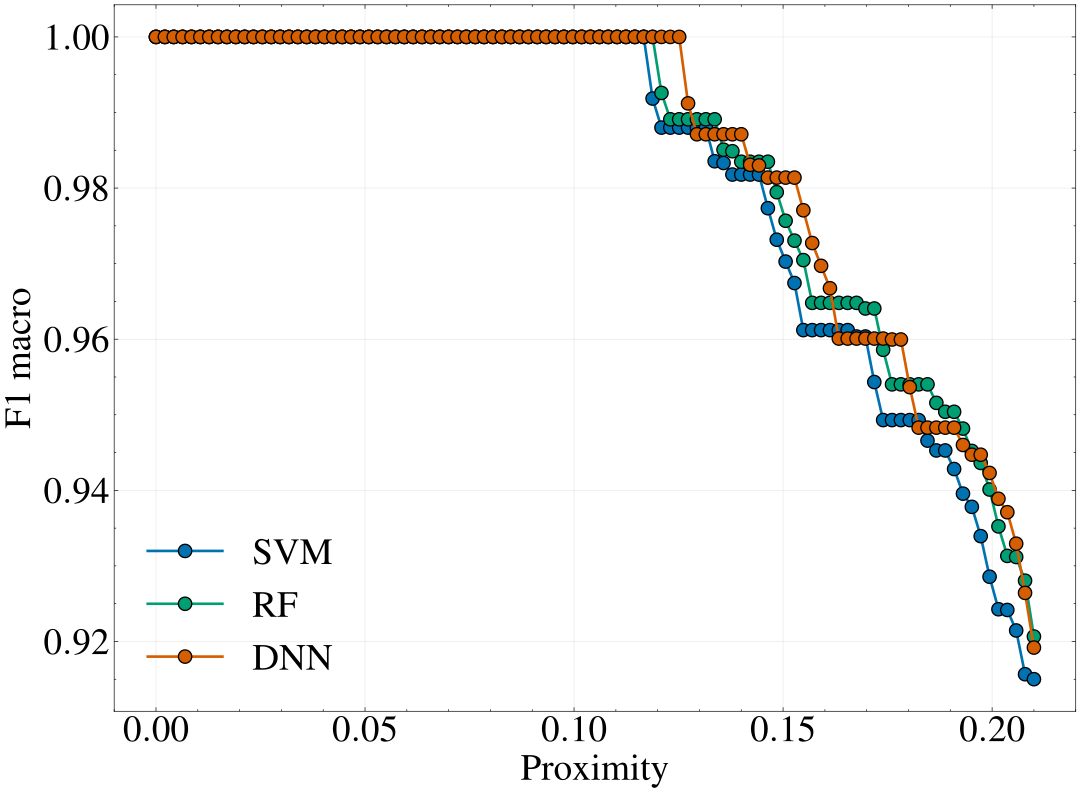
\includegraphics[width=0.95\linewidth]{sections/TATA/results/figures/proximity_in_practice-transparent.png}
			\caption{\scriptsize Macro-F1 vs. proximity across cumulative sub-tests (IDS2017).}
		\end{figure}
	\end{columns}
\end{frame}


%%================= DIVERSITY (in practice) =================
%\begin{frame}{Diversity in Practice (IDS2017 only)}
%  \small
%  \begin{columns}[T,onlytextwidth]
%    % Left: text
%    \column{0.58\linewidth}
%    \begin{itemize}
%      \item Sub-test sets: all label combinations of size \(k=1\ldots9\).
%      \item Diversity rises monotonically with \(k\); maximum \(\approx 0.1209\).
%      \item More traffic types \(\Rightarrow\) higher diversity \(\Rightarrow\)
%      more challenging evaluation.
%    \end{itemize}
%
%    % Right: figure
%    \column{0.40\linewidth}
%    \centering
%    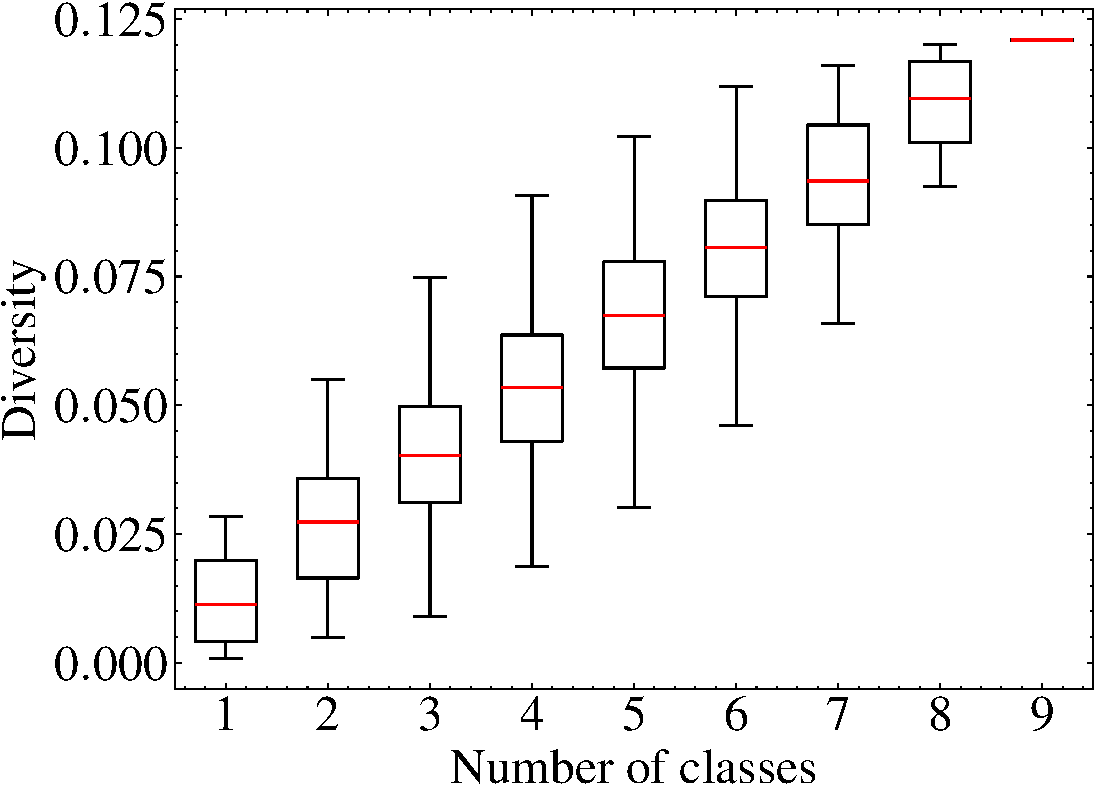
\includegraphics[width=\linewidth]{results/figures/diversity_boxplot-crop}
%  \end{columns}
%\end{frame}

%%================= SCARCITY (in practice) =================
%\begin{frame}{Scarcity in Practice (IDS2017 only)}
%  \small
%  \begin{columns}[T,onlytextwidth]
%    % Left: text
%    \column{0.58\linewidth}
%    \begin{itemize}
%      \item Increase scarcity by redistributing misclassified points across all negative
%      clusters in 10 steps.
%      \item
%      Macro-F1 drops sharply then monotonically; strong negative correlation; For
%      example, RF \(<0.78\) at scarcity \(\approx 0.53\).
%      \item More uniform spread across boundaries \(\Rightarrow\) higher scarcity
%      \(\Rightarrow\) lower macro-F1.
%    \end{itemize}
%
%    % Right: figure
%    \column{0.40\linewidth}
%    \centering
%    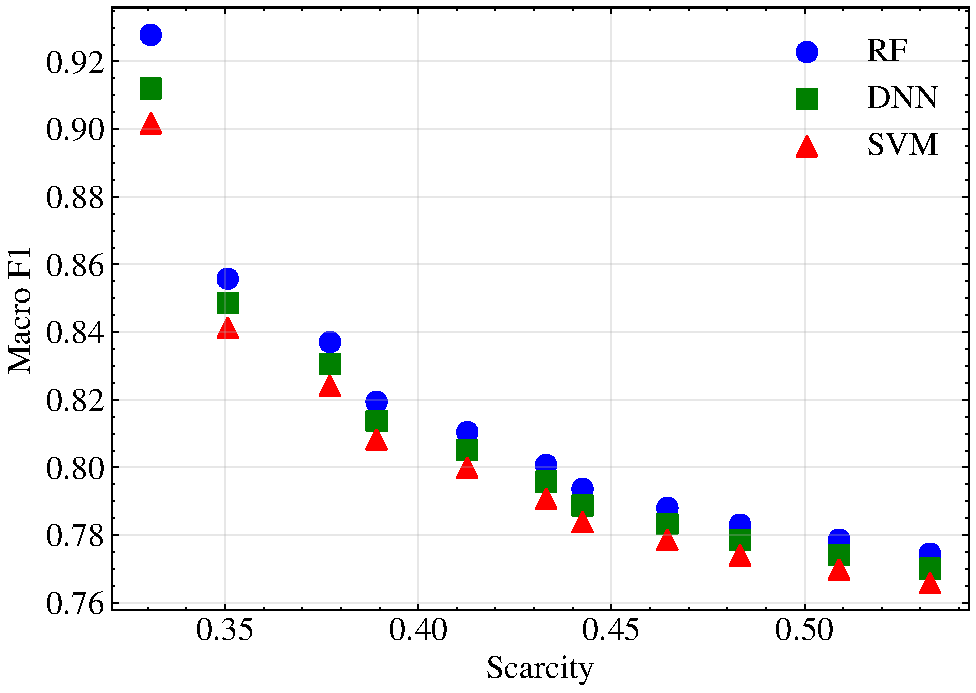
\includegraphics[width=0.95\linewidth]{results/figures/scarcity_in_practice}
%  \end{columns}
%\end{frame}

%\begin{frame}
%{Test set Augmentation Evaluation}
%
%  \scriptsize
%  \begin{columns}[T,onlytextwidth]
%    \column{0.55\linewidth}
%    \begin{itemize}
%      \item \textbf{Protocol:}
%      20 eval episodes on IDS2017; no reward/updates; add Benign SSH flows;
%      report mean$\pm$sd.
%      \item \textbf{Baselines:} Random, NetShare (GAN), RL\,+\,
%      Neuron Coverage (NC).
%      \item \textbf{Quality metrics:}
%      \begin{itemize}
%        \scriptsize
%        \item \textbf{TATA:} \(D\) \textcolor{green!60!black}{\(+\sim 437\%\)};
%        \(P\) \textcolor{green!60!black}{\(+\sim 190\%\)};
%        \(S\) \textcolor{green!60!black}{\(+\sim 136\%\)}
%        \item \textbf{NC:} \(D\) \textcolor{gray!60!black}{\(\approx 0\)};
%        \(P\) \textcolor{green!60!black}{\(+\sim 129\%\)};
%        \(S\) \textcolor{gray!60!black}{\(\approx 0\)}
%        \item \textbf{Random/NetShare:} \(D\)
%        \textcolor{red!70!black}{\(\downarrow\) to \(\approx 0\)};
%        \(P\) \textcolor{gray!60!black}{\(\approx 0\)};
%        \(S\) \textcolor{red!70!black}{\(\downarrow\)}
%      \end{itemize}
%
%      \item \textbf{NIDS impact:}
%      \begin{itemize}
%        \scriptsize
%        \item \textbf{TATA (RF example):} Precision
%        \textcolor{red!70!black}{–$\sim$46\%}; Recall
%        \textcolor{red!70!black}{–$\sim$13\%}
%        \item \textbf{NC (RF example):} Precision
%        \textcolor{red!70!black}{–$\sim$23\%}; Recall
%        \textcolor{red!70!black}{–$\sim$16\%}
%        \item \textbf{Note:} higher scarcity spreads errors across boundaries
%        $\Rightarrow$ FP $\uparrow$ $\Rightarrow$ precision $\downarrow$.
%      \end{itemize}
%
%    \end{itemize}
%
%    \column{0.42\linewidth}
%    \centering
%    \begin{figure}
%      \includegraphics[width=\linewidth]
%      {results/figures/bars_classifier_grayscale_std}
%      \caption*{\scriptsize
%      {Impact of TATA and Baselines on Test-Set Quality Metrics and Detection
%      Performance}}
%      \label{fig:test_set_aug_1}
%    \end{figure}
%  \end{columns}
%
%\end{frame}



\begin{frame}{Test-set Augmentation — Metrics}
	\small
	\begin{columns}[T,onlytextwidth]
		% ---------------- Left column ----------------
		\column{0.55\linewidth}
		\begin{itemize}
			\item<1-> \textbf{Protocol:}
			      20 eval episodes on IDS2017; no reward/updates; add Benign SSH flows;
			      report mean$\pm$sd.

			\item<1-> \textbf{Baselines:} Random, NetShare (GAN), RL\,+\,Neuron Coverage (NC).

			\item<2-> \textbf{Quality metrics:}
			      \begin{itemize}
				      \item<2-> \textbf{TATA:} \(D\) \textcolor{green!60!black}{\(+\sim 437\%\)}; \(P\)
				            \textcolor{green!60!black}{\(+\sim 190\%\)}; \(S\)
				            \textcolor{green!60!black}{\(+\sim 136\%\)}
				      \item<2-> \textbf{NC:} \(D\) \textcolor{gray!60!black}{\(\approx 0\)}; \(P\)
				            \textcolor{green!60!black}{\(+\sim 129\%\)}; \(S\)
				            \textcolor{gray!60!black}{\(\approx 0\)}
				      \item<2-> \textbf{Random/NetShare:} \(D\)
				            \textcolor{red!70!black}{\(\downarrow\) to \(\approx 0\)}; \(P\)
				            \textcolor{gray!60!black}{\(\approx 0\)}; \(S\)
				            \textcolor{red!70!black}{\(\downarrow\)}
			      \end{itemize}
		\end{itemize}

		% Step 3: prompt to transition
		\only<3->{%
			\begin{beamercolorbox}[rounded=true,shadow=true,wd=\linewidth,sep=0.8ex]{focusbox}
				\normalsize What is the impact on NIDS performance?
			\end{beamercolorbox}
		}

		% ---------------- Right column ----------------
		\column{0.42\linewidth}
		\centering
		\begin{figure}
			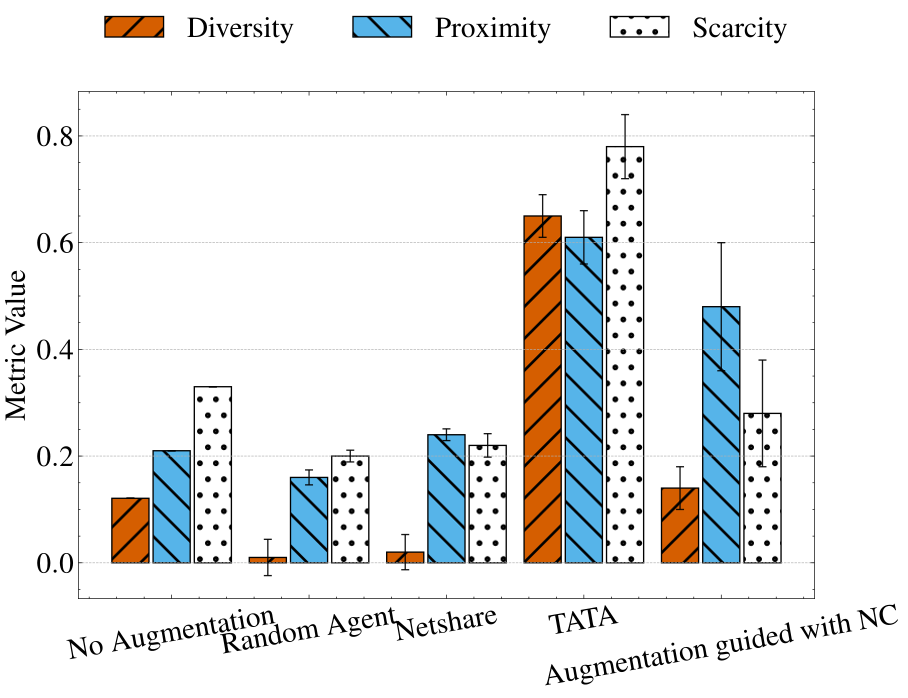
\includegraphics[width=\linewidth]{sections/TATA/results/figures/metrics_bars_grayscale_std-transparent.png}
			\caption{\scriptsize Test-set quality metrics (higher is more challenging/covered).}
			\label{fig:aug}
		\end{figure}
	\end{columns}
\end{frame}


\begin{frame}{Test-set Augmentation — Impact on NIDS}
	\small
	\begin{columns}[T,onlytextwidth]
		% ---------------- Left column ----------------
		\column{0.55\linewidth}
		\begin{itemize}
			\item \textbf{NIDS impact (RF example):}
			      \begin{itemize}

				      \item \textbf{TATA:} Precision \textcolor{red!70!black}{--\(\sim\)46\%}; Recall
				            \textcolor{red!70!black}{--\(\sim\)13\%}
				      \item[]
				      \item \textbf{NC:} Precision \textcolor{red!70!black}{--\(\sim\)23\%}; Recall
				            \textcolor{red!70!black}{--\(\sim\)16\%}
			      \end{itemize}
			\item[]
			\item \textbf{Note:} higher scarcity spreads errors across boundaries
			      \(\Rightarrow\) FP \(\uparrow\) \(\Rightarrow\) precision \(\downarrow\).
			\item[]
			\item \(\Rightarrow\) \textbf{proximity is the key driver;}
			      scarcity and diversity are complementary (spread errors, avoid redundancy)

		\end{itemize}

		% ---------------- Right column ----------------
		\column{0.42\linewidth}
		\centering
		\begin{figure}
			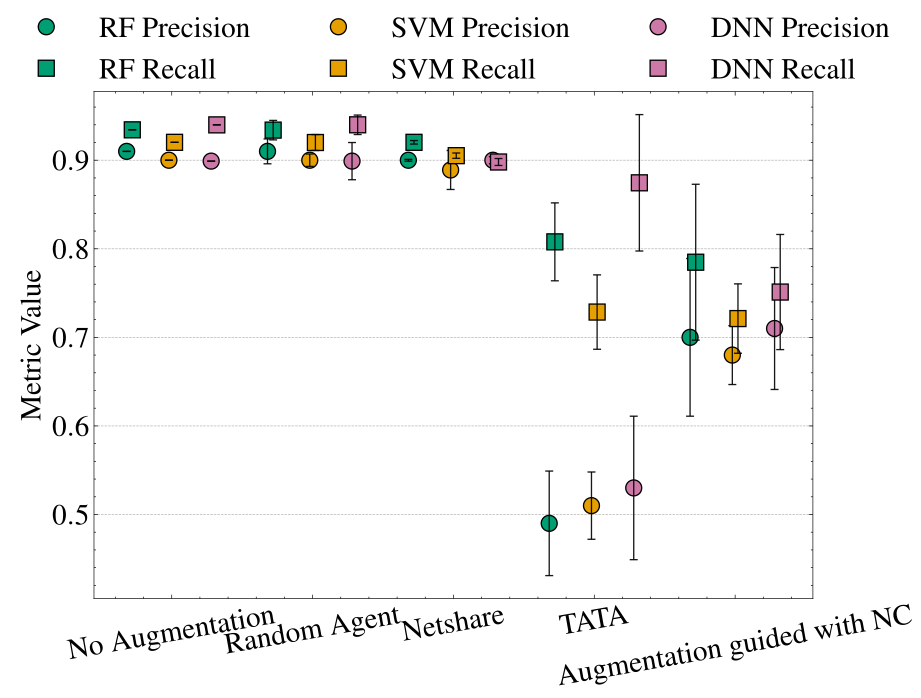
\includegraphics[width=\linewidth]{sections/TATA/results/figures/nids_performance_grayscale_std-transparent.png}
			\caption{\scriptsize Impact on detection metrics (example: RF).}\label{fig:figure}
		\end{figure}
	\end{columns}
\end{frame}


%\begin{frame}{Test-set Augmentation Evaluation}
%  \scriptsize
%  \begin{columns}[T,onlytextwidth]
%    % ---------------- Left column (adds content over time) ----------------
%    \column{0.55\linewidth}
%    \begin{itemize}
%      \item<1-> \textbf{Protocol:}
%      20 eval episodes on IDS2017; no reward/updates; add Benign SSH flows;
%      report mean$\pm$sd.
%
%      \item<1-> \textbf{Baselines:} Random, NetShare (GAN), RL\,+\,Neuron Coverage (NC).
%
%      \item<2-> \textbf{Quality metrics:}
%      \begin{itemize}
%        \scriptsize
%        \item<2-> \textbf{TATA:} \(D\) \textcolor{green!60!black}{\(+\sim 437\%\)}; \(P\)
%        \textcolor{green!60!black}{\(+\sim 190\%\)}; \(S\)
%        \textcolor{green!60!black}{\(+\sim 136\%\)}
%        \item<2-> \textbf{NC:} \(D\) \textcolor{gray!60!black}{\(\approx 0\)}; \(P\)
%        \textcolor{green!60!black}{\(+\sim 129\%\)}; \(S\)
%        \textcolor{gray!60!black}{\(\approx 0\)}
%        \item<2-> \textbf{Random/NetShare:} \(D\)
%        \textcolor{red!70!black}{\(\downarrow\) to \(\approx 0\)}; \(P\)
%        \textcolor{gray!60!black}{\(\approx 0\)}; \(S\)
%        \textcolor{red!70!black}{\(\downarrow\)}
%      \end{itemize}
%
%      \item<3-> \textbf{NIDS impact:}
%      \begin{itemize}
%        \scriptsize
%        \item<3-> \textbf{TATA (RF example):} Precision
%        \textcolor{red!70!black}{--\(\sim\)46\%}; Recall
%        \textcolor{red!70!black}{--\(\sim\)13\%}
%        \item<3-> \textbf{NC (RF example):} Precision
%        \textcolor{red!70!black}{--\(\sim\)23\%}; Recall
%        \textcolor{red!70!black}{--\(\sim\)16\%}
%        \item<3-> \textbf{Note:} higher scarcity spreads errors across boundaries
%        \(\Rightarrow\) FP \(\uparrow\) \(\Rightarrow\) precision \(\downarrow\).
%      \end{itemize}
%    \end{itemize}
%
%    % ---------------- Right column (figure swaps on step 3) ----------------
%    \column{0.42\linewidth}
%    \centering
%    \only<1-2>{%
%      \begin{figure}
%        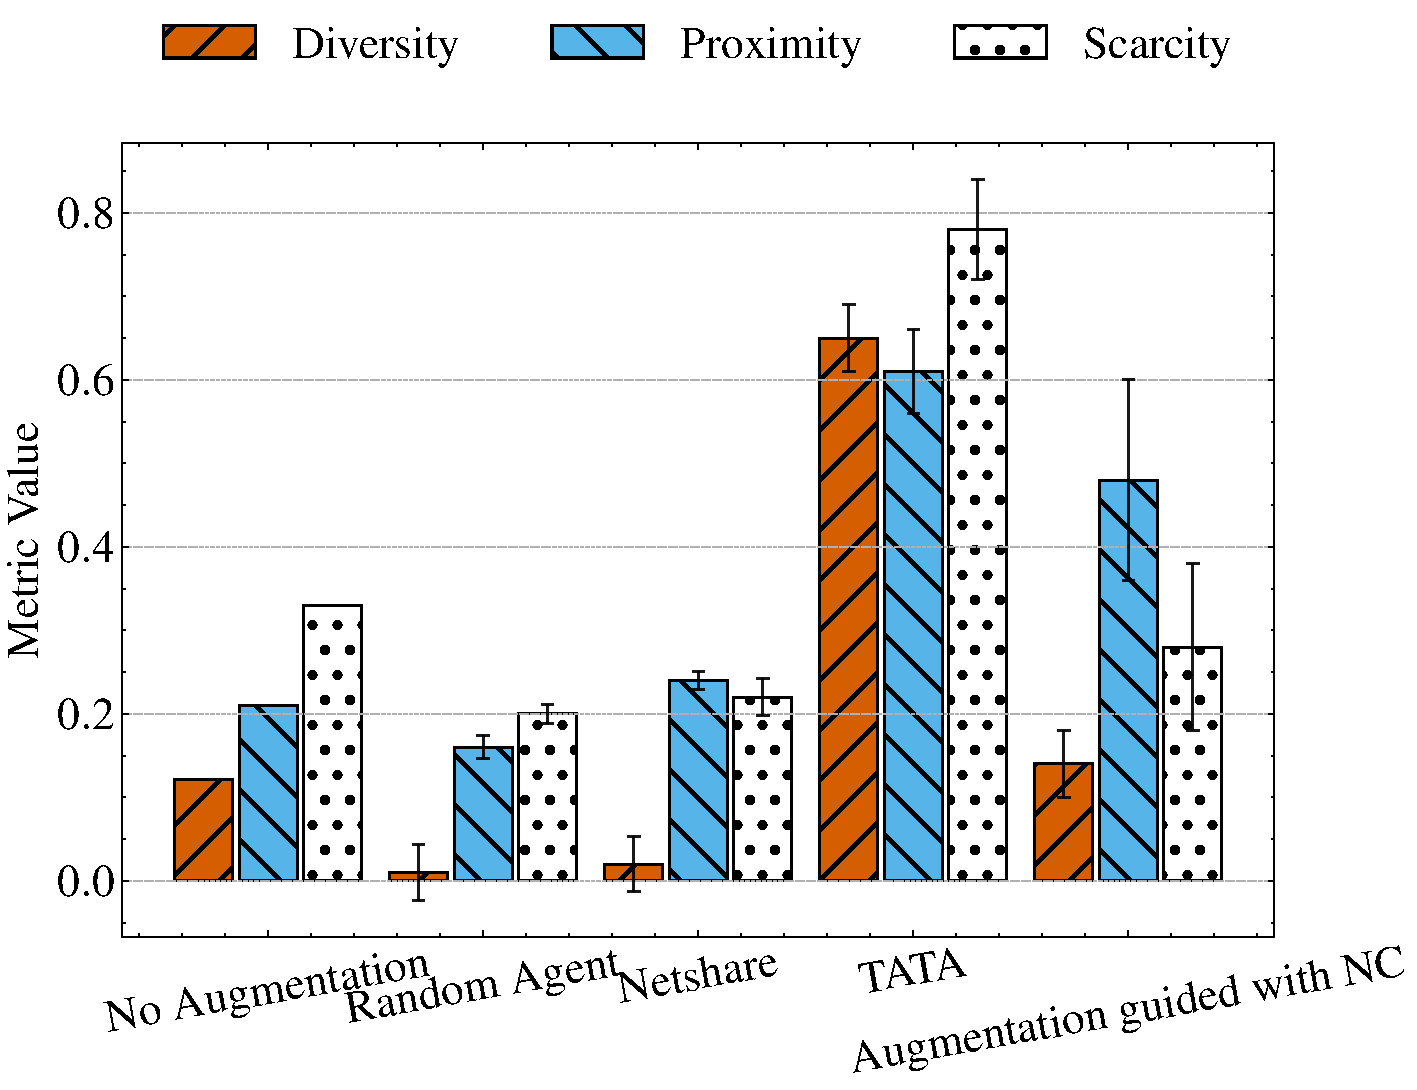
\includegraphics[width=\linewidth]{results/figures/metrics_bars_grayscale_std}
%        \label{fig:test_set_aug_metrics}
%      \end{figure}
%    }
%    \only<3->{%
%      \begin{figure}
%        \includegraphics[width=\linewidth]
%        {results/figures/nids_performance_grayscale_std}% <-- replace with your impact
%        \label{fig:test_set_aug_impact}
%      \end{figure}
%    }
%  \end{columns}
%\end{frame}
%\begin{frame}{Test-set Augmentation Evaluation}
%  \scriptsize
%  \begin{columns}[T,onlytextwidth]
%    % ---------------- Left column ----------------
%    \column{0.55\linewidth}
%
%    % (1) Protocol + Baselines
%    \only<1>{
%      \textbf{Protocol:} 20 eval episodes on IDS2017; no reward/updates; add Benign SSH
%      flows; report mean$\pm$sd.\\[0.4em]
%      \textbf{Baselines:} Random, NetShare (GAN), RL\,+\,Neuron Coverage (NC).
%    }
%
%    % (2) Quality metrics
%    \only<2>{
%      \textbf{Quality metrics:}
%      \begin{itemize}
%        \scriptsize
%        \item \textbf{TATA:} \(D\) \textcolor{green!60!black}{\(+\sim 437\%\)};\; \(P\)
%        \textcolor{green!60!black}{\(+\sim 190\%\)};\; \(S\)
%        \textcolor{green!60!black}{\(+\sim 136\%\)}
%        \item \textbf{NC:} \(D\) \textcolor{gray!60!black}{\(\approx 0\)};\; \(P\)
%        \textcolor{green!60!black}{\(+\sim 129\%\)};\; \(S\)
%        \textcolor{gray!60!black}{\(\approx 0\)}
%        \item \textbf{Random/NetShare:} \(D\)
%        \textcolor{red!70!black}{\(\downarrow\) to \(\approx 0\)};\; \(P\)
%        \textcolor{gray!60!black}{\(\approx 0\)};\; \(S\)
%        \textcolor{red!70!black}{\(\downarrow\)}
%      \end{itemize}
%    }
%
%    % (3) NIDS impact
%    \only<3>{
%      \textbf{NIDS impact:}
%      \begin{itemize}
%        \scriptsize
%        \item \textbf{TATA (RF example):} Precision
%        \textcolor{red!70!black}{--\(\sim\)46\%};\; Recall
%        \textcolor{red!70!black}{--\(\sim\)13\%}
%        \item \textbf{NC (RF example):} Precision \textcolor{red!70!black}{--\(\sim\)
%23\%}
%        ;\; Recall \textcolor{red!70!black}{--\(\sim\)16\%}
%        \item \textbf{Note:} higher scarcity spreads errors across boundaries
%        \(\Rightarrow\) FP \(\uparrow\) \(\Rightarrow\) precision \(\downarrow\).
%      \end{itemize}
%    }
%
%    % ---------------- Right column ----------------
%    \column{0.42\linewidth}
%    \centering
%    \only<1-2>{%
%      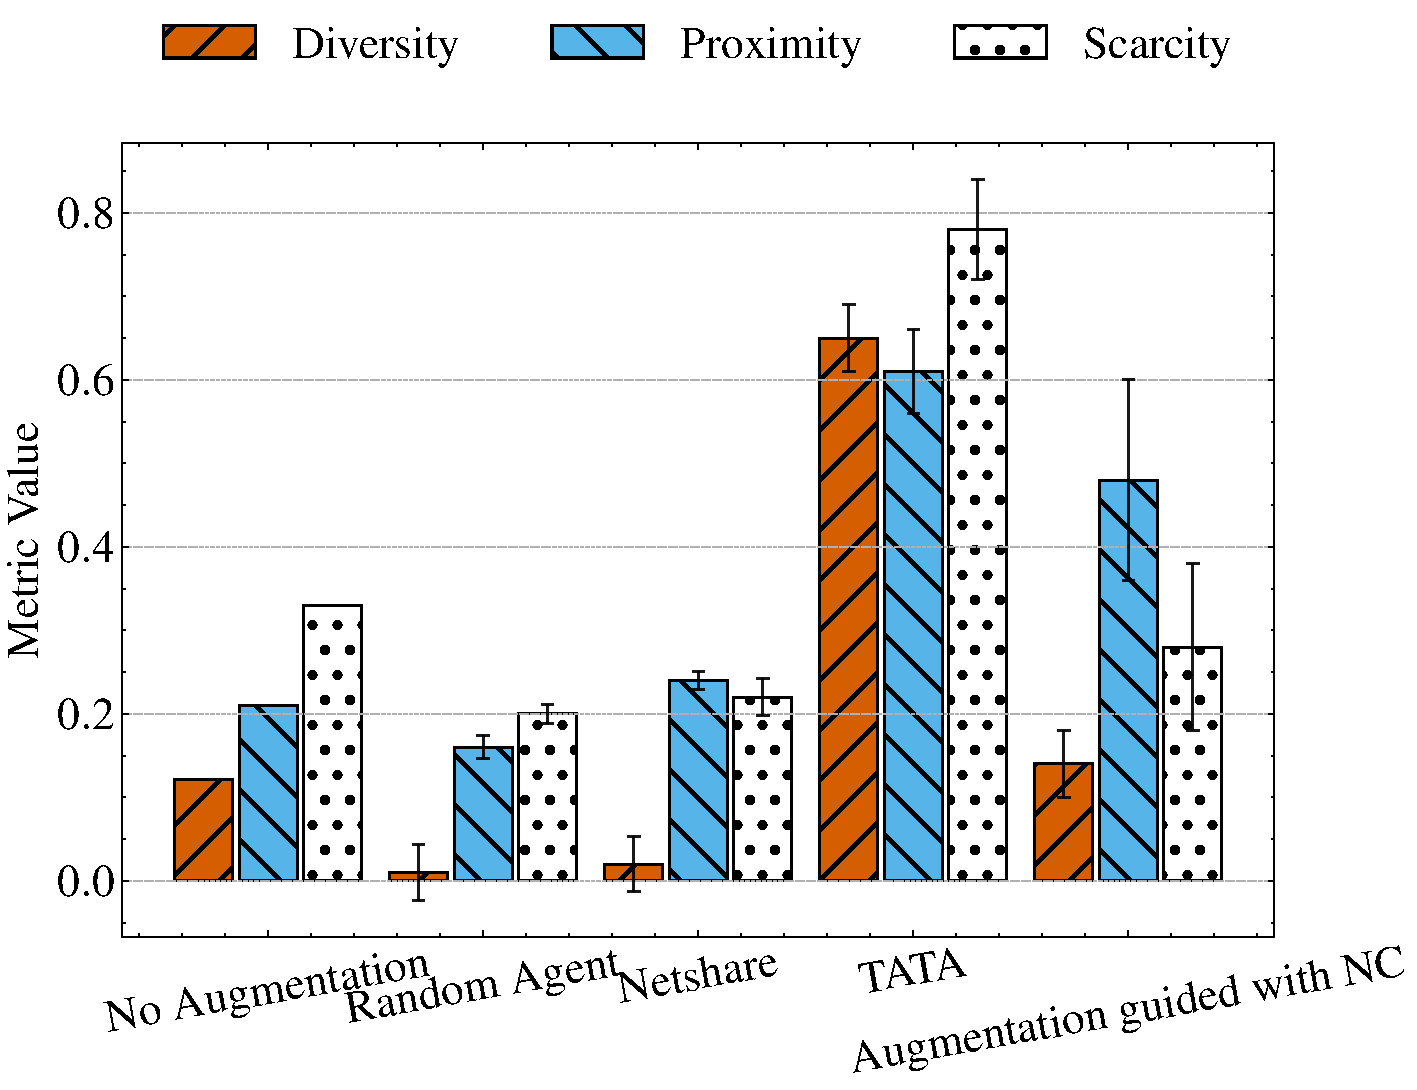
\includegraphics[width=\linewidth]{results/figures/metrics_bars_grayscale_std}%
%    }
%    \only<3->{%
%      \includegraphics[width=\linewidth]
%      {results/figures/nids_performance_grayscale_std}
%    }
%  \end{columns}
%\end{frame}


%\begin{frame}
%{Test set Augmentation Evaluation}
%
%
%  \small
%  \begin{columns}[T,onlytextwidth]
%    \column{0.55\linewidth}
%    \begin{itemize}
%      \item \textbf{Reward ablation:} train with single metrics or pairs: \(D\),
%      \(P\), \(S\), \(D{+}P\), \(P{+}S\), \(S{+}D\).
%      \item \textbf{Result:} any combo including \(P\) (\(P\), \(P{+}S\),
%      \(D{+}P\)) stresses NIDS most; others have minor impact.
%      \item \textbf{Example (RF):} \(P{+}S\) → recall \(0.934\!\to\!0.862\) (
%      \(-\sim8\%\)), precision \(0.910\!\to\!0.460\) (\(-\sim49\%\)); \(S{+}D\)
%      → recall \(-\sim4\%\), precision \(-\sim3\%\).
%      \item \textbf{Takeaway:} \(P\) is the key driver; \(S,D\)
%      are complementary (spread errors, avoid redundancy).
%    \end{itemize}
%
%    \column{0.42\linewidth}
%    \centering
%    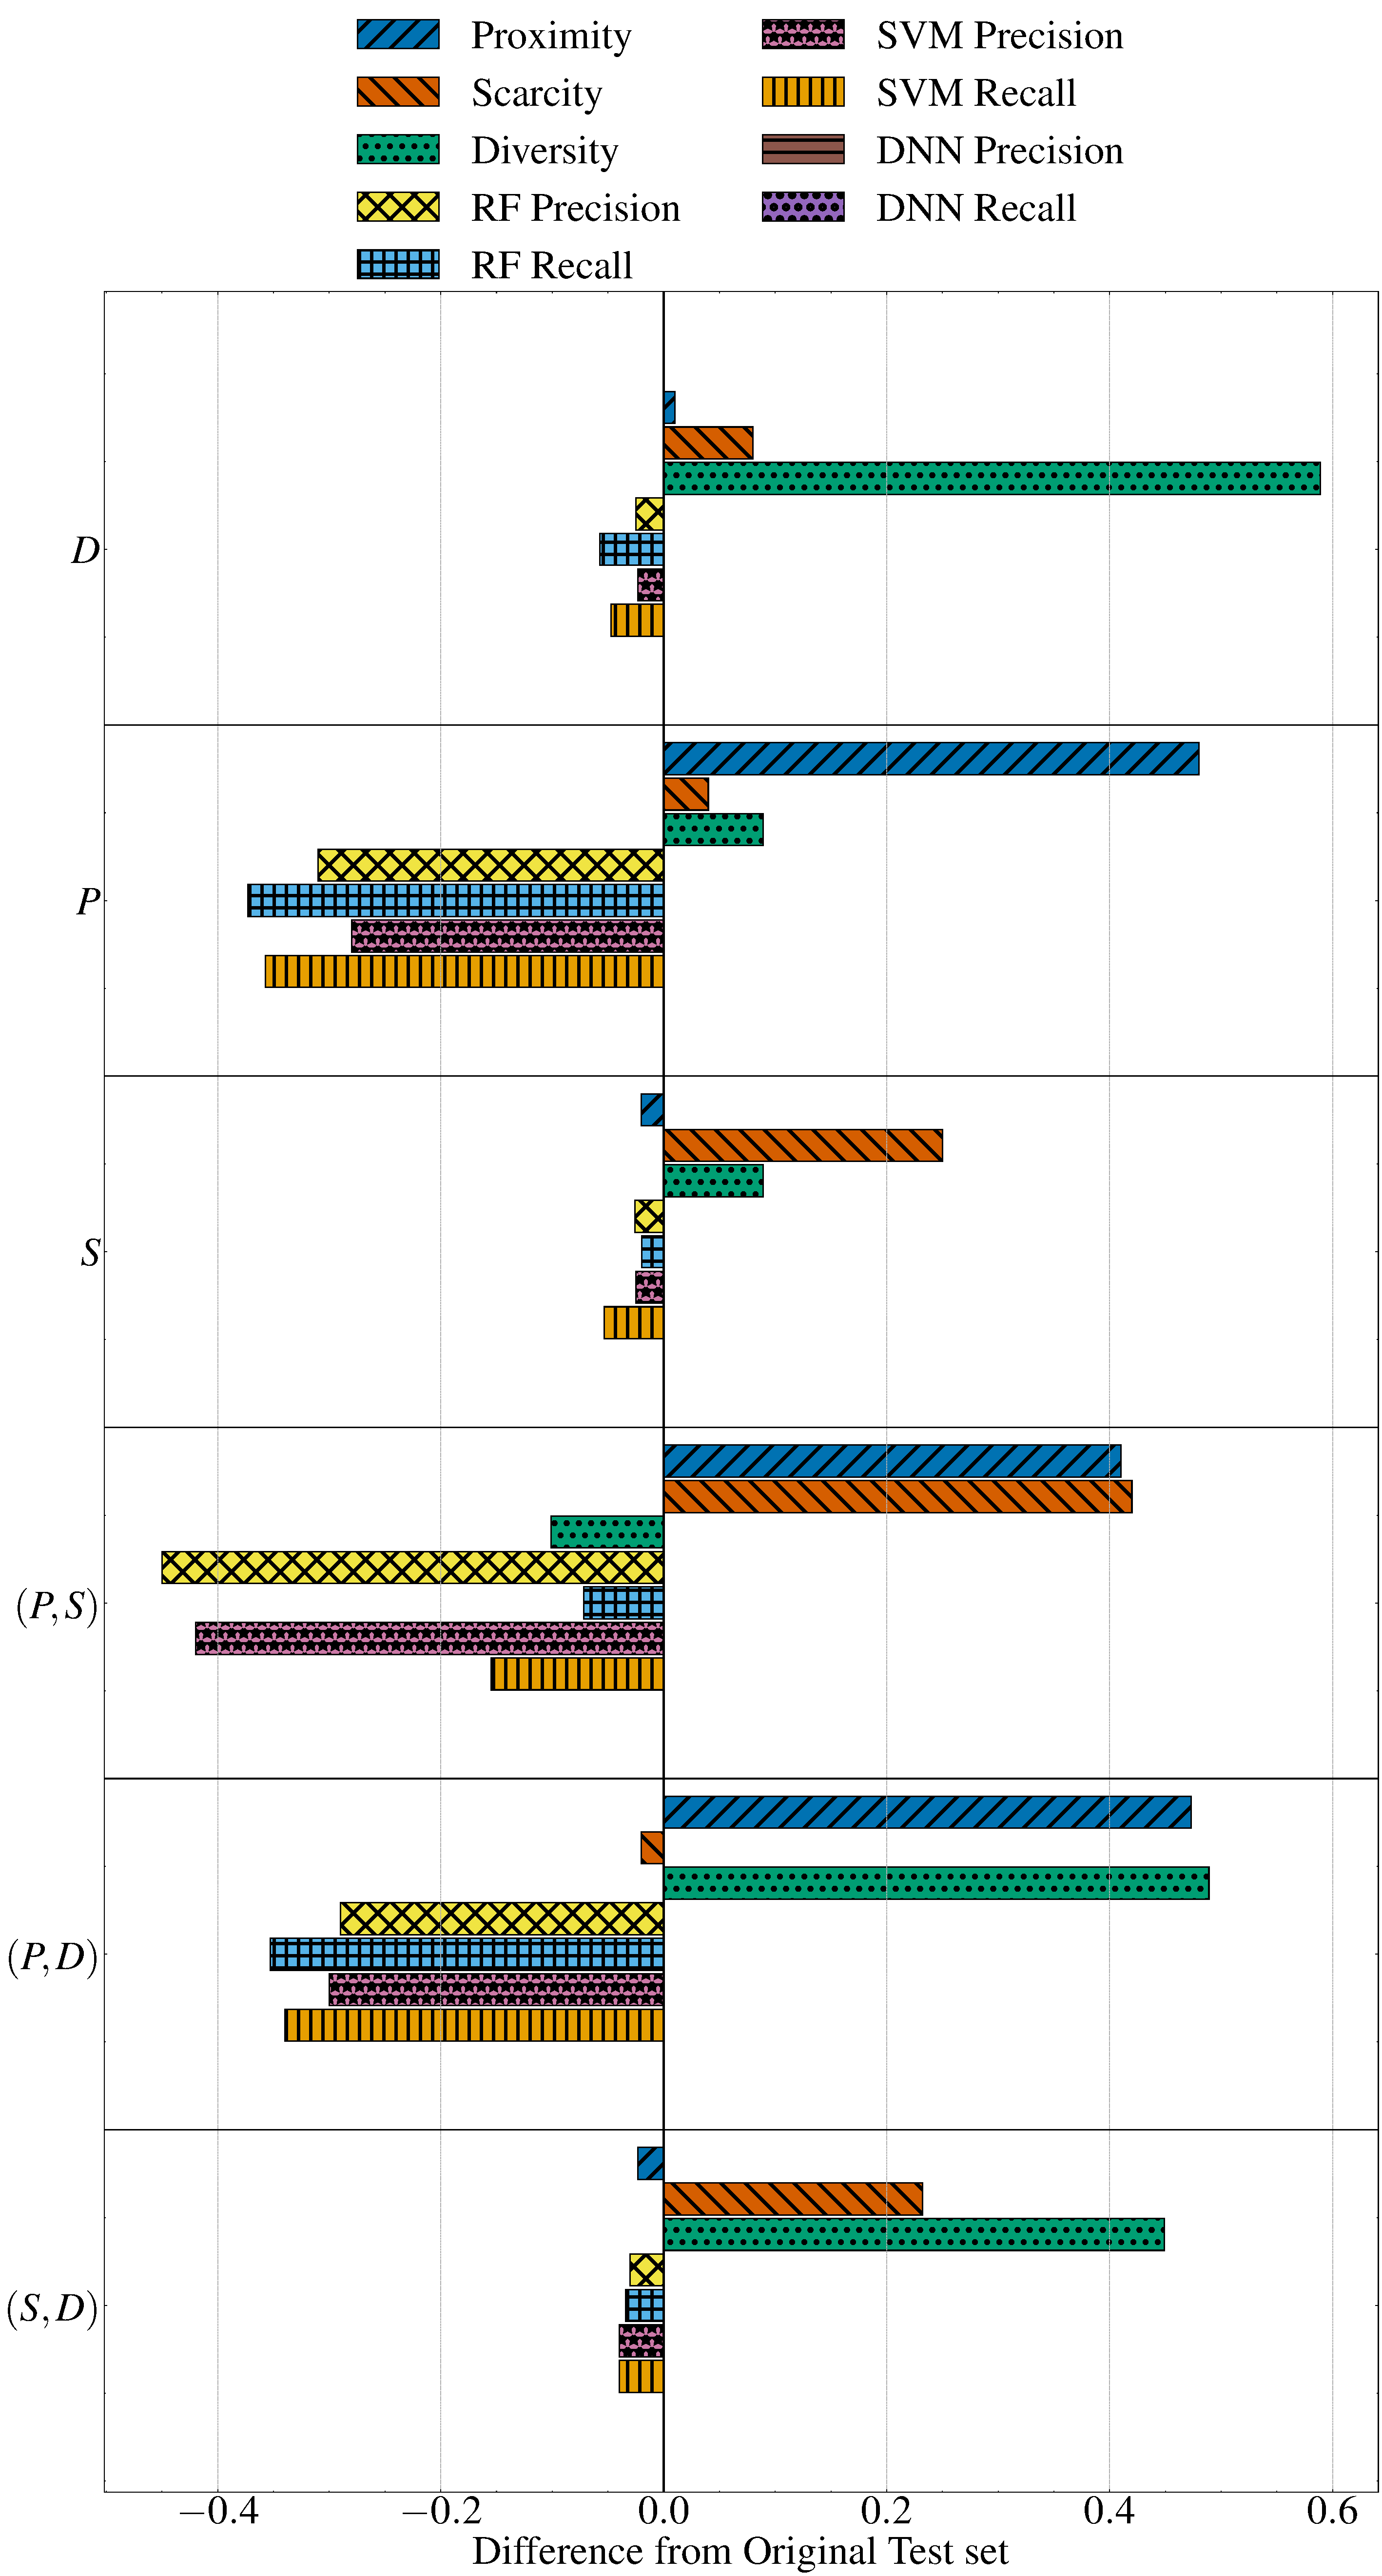
\includegraphics[width=0.7\linewidth]{results/figures/centered_bars_diff}
%  \end{columns}
%
%\end{frame}

\begin{frame}{Datasets Analysis}

	\small
	\begin{columns}[T,onlytextwidth]
		\column{0.55\linewidth}
		\begin{itemize}
			\item Apply \(D,P,S\)
			      across many NIDS datasets (2009–2020), sorted by release year; averages
			      over ten 60/20 splits.
			\item []
			\item No increasing pattern; values mostly \(\le 0.5\)
			      with occasional peaks (e.g., early IDS2017/2018); low within-dataset variation.
			\item []
			\item \(\Rightarrow\)
			      Despite richer, newer testbeds, NIDS test-set difficulty hasn’t
			      substantially increased. (CV refs like MNIST/CIFAR-10 score higher on
			      \(D,P,S\).)
		\end{itemize}
		\column{0.42\linewidth}
		\begin{figure}
			\centering
			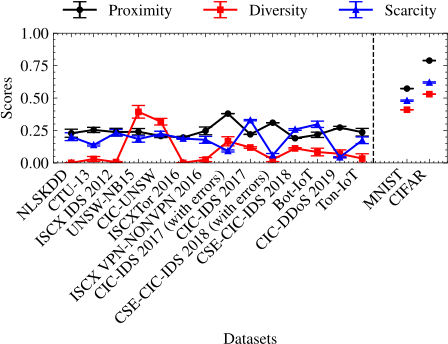
\includegraphics[width=\linewidth]{sections/TATA/results/figures/datasets_analysis-crop-transparent.png}
			\caption{\scriptsize Test-set assessment of NIDS datasets.}
			\label{fig:datasets_analysis}
		\end{figure}
	\end{columns}

\end{frame}
